\documentclass[../../szobeli.tex]{subfiles}

\begin{document}

\begin{center}
    \noindent\fbox{%
    	\parbox{160mm}{
			\textbf{Euler-séta és körséta} \underline{létezésének szükséges és elégséges feltétele}. \textbf{Hamilton-kör és út} létezésére szükséges, ill. elégséges feltételek: \underline{komponensszám ponttörlés után} (Petersen-gráf) \underline{\textbf{Dirac, Ore tételei}}, gazdag párok, \underline{hízlalási lemma}, Chavátal-lezárt.
        }
    }
\end{center}

    \begin{itemize}
        \item \textbf{Euler-séták}

        \textcolor{blue}{\textbf{Def:}} A $G$ gráf \textcolor{red}{Euler-(kör)sétája} a $G$ egy olyan (kör)sétája, ami $G$ minden élét tartalmazza.

        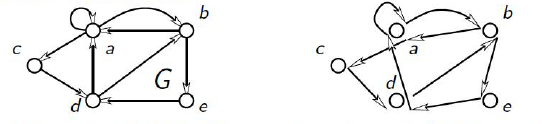
\includegraphics[width=\textwidth]{img/1.png}

        \textcolor{blue}{\textbf{Megj:}} \begin{itemize}
            \item[(1)] A fenti definíció 2 $\times$ 2 fogalmat definiál: az Euler-sétát és az Euler-körsétát irányítatlan és irányított gráfra is. 
            \item[(2)] Szokás a definíciót abban a formában kimondani, hogy az Euler-(kör)séta $G$ minden élét \textbf{pontosan} egyszer tartalmazza. Tekintettel arra, hogy egy séta nem mehet át kétszer ugyanazon az élen, ez redundáns kivánalom, hiszen következménye az általunk használt definíciónak. Használatos ezen kívül az Euler-kör ill. Euler-út megnevezés is a fenti fogalmakra. 
            \item[(3)] Irányítatlan Euler-séta: "$G$ egy vonallal lerajzolható".
        \end{itemize}

        \textcolor{green}{\textbf{Cél:}} Gyors módszer az Euler-(kör)séta megtalálására, létezésének ellenőrzésére.

        \textcolor{orange}{\textbf{Megf:}} (1) Ha a $G$ irányított gráfnak van Euler-körsétája, akkor 

            (a) $G$ izolált pontoktól eltekintve gyengén összefüggő, és 

            (b) minden $v$ csúcsára $\rho(v) = \delta(v)$ teljesül.

        \textcolor{green}{\textbf{Biz:}} (a) Ha $G$ két különböző gyenge komponense is tartalmaz élt, akkor $G$-nek nem lehet Euler-körsétája, hisz egyetlen séta sem tartalmazhat élt két különböző gyenge komponensből. \checkmark

        (b) Ha végighaladunk az Euler-körsétán, akkor a $v$ csúcsba pontosan annyiszor lépünk be, mint ahányszor kilépünk onnan. A körséta $G$ minden élét pontosan egyszer érinti: $\rho(v) = \delta(v)$   

        \textcolor{orange}{\textbf{Megf:}} (2) Ha a $G$ irányítatlan gráfnak van Euler-körsétája, akkor 

            (a) $G$ izolált pontoktól eltekintve összefüggő, és

            (b) $G$-ben minden fokszám páros.

        \textcolor{green}{\textbf{Biz:}} Az irányított esethez hasonló. (a) Egy (kör)séta nem tartalmazhatja két különböző komponensnek is $1-1$ élét, és (b) az Euler-körsétát követve tetszőleges $v$ csúcsba ugyanyannyiszor lépünk be, mint ahányszor kilépünk belőle. Ezért $d(v)$ páros.   

        \textcolor{orange}{\textbf{Megf:}} (3) Ha a $G$ irányítatlan gráfnak van Euler-sétája, akkor 

            (a) $G$ izolált pontoktól eltekintve összefüggő, és

            (b) $G$-nek 0 vagy 2 páratlan fokú csúcsa van.

        \textcolor{green}{\textbf{Biz:}} (a) \checkmark. (b): Tegyük fel, hogy $G$ Euler-sétája egy $uv$-séta. Ekkor minden $w \neq u,v$ csúcsra $d(w)$ kétszer annyi, mint ahányszor az Euler-séta $w$-n áthalad, vagyis $d(w)$ páros. Ha $u = v$, akkor az Euler-séta körséta, így $d(u)$ is páros (2b) miatt. Ha pedig $u \neq v$, akkor $u$-ból 1-gyel többször lépünk ki, mint be, v-be 1-gyel többször lépünk be, mint ki, vagyis $d(u)$ és $d(v)$ páratlanok.  

        \textcolor{blue}{\textbf{Megj:}} A fenti megfigyelés segítségével bizonyos esetekben azonnal látszik, hogy $G$-nek nincs Euler-sétája ill. -körsétája.

        $G$ \textcolor{red}{irányítatlan Euler-gráf}, ha $G$ minden $v$ csúcsra $d(v)$ páros.

        \textcolor{orange}{\textbf{Lemma:}} Ha $G$ Euler-gráf, akkor $G$ élei kiszínezhetők úgy, hogy az egyszínű élek (irányított) kört alkossanak minden színre.

        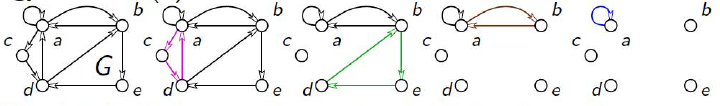
\includegraphics[width=\textwidth]{img/2.png}

        \textcolor{green}{\textbf{Biz:}} Induljunk el $G$ egy éle mentén, és haladjunk tovább az (irányított) élek mentén. Mivel $G$ Euler, ezért sosem akadunk el: előbb-utóbb ismétlődik egy csúcs, így találunk egy $C_1$ kört. $C_1$ éleit törölve $G-C_1$ Euler-gráf marad. Ismételjük meg ezt a $G-C_1$ gráfon. Így $G$ minden éle előbb-utóbb sorra kerül és megkapja a $C_2, C_3, \dots$ köröket. Ezért $E(G) = C_1 \cup C_2 \cup \dots$ diszjunkt körök uniójára bomlik fel. Színezzük ki a $C_1$ kör éleit az $i$-dik színnel.  

        \textcolor{orange}{\textbf{Tétel:}} (1) ($G$ irányított gráfnak van Euler-körsétája) $\Longleftrightarrow$ ($G$ Euler-gráf és $G$ izolált pontoktól eltekintve gyengén összefüggő) 
        
        (2) ($G$ irányítatlan gráfnak van Euler-körsétája) $\Longleftrightarrow$ ($G$ Euler-gráf és $G$ izolált pontoktól eltekintve összefüggő)

        \textcolor{green}{\textbf{Biz:}} $\Rightarrow$: Láttuk. \checkmark $\Leftarrow$: A Lemma miatt $E(G)$ felbontható körökre, tehát körsétákra is. Ha a körséták száma legalább 2, akkor választunk két körsétát, aminek van közös csúcsa és $e$ csúcs mentén "összevarjuk" azokat. Mindezt addig végezzük, amíg egyetlen körséta marad.  

        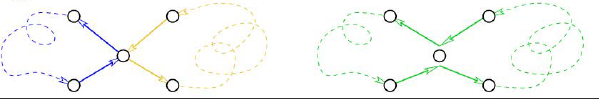
\includegraphics[width=\textwidth]{./img/3.png}

        \textcolor{orange}{\textbf{Tétel:}} (3) ($G$ irányítatlan gráfnak van Euler-sétája) $\Longleftrightarrow$ ($G$ izolált pontoktól eltekintve összefüggő és 0 vagy 2 páratlan fokú csúcsa van.)

        \textcolor{green}{\textbf{Biz:}} $\Rightarrow$: Láttuk. \checkmark $\Leftarrow$: Ha $G$ Euler-gráf, akkor (2) miatt van Euler-körsétája, ami Euler-séta is egyúttal. Ha $G$ nem Euler-gráf, akkor legyenek $u$ és $v$ a $G$ páratlan fokú csúcsai. Ekkor $G + uv$ Euler-gráf, és (2) miatt van Euler-körsétája. Feltehető, hogy $e$ körséta utolsó éle $uv$. Ezt az $uv$ élt elhagyva a körsétából, $G$ Euler-sétáját kapjuk. 

        \textcolor{violet}{\textbf{Euler-körséta keresése Euler-gráfban:}} $E(G)$-t felbontjuk körsétákra, amiket összevarrunk. Körsétát a felbontáshoz pl. úgy is kereshetünk, hogy addig követünk egy sétát, amíg tudunk. Előbb-utóbb elakadunk, de ez csakis a séta kiindulási pontjában történhet meg. Ezért a bejárt séta egy körséta, amit a felbontásban felhasználunk.

        \item \textbf{Hamilton-körök és -utak} 

        \textcolor{blue}{\textbf{Def:}} A $G$ gráf \textcolor{red}{Hamilton-köre} (\textcolor{red}{Hamilton-útja}) a $G$ olyan köre (útja), ami $G$ minden csúcsát tartalmazza. 

        \textcolor{blue}{\textbf{Megj:}} A célunk hasonló, mint az Euler-(kör)séta esetén, azaz gyors módszer, amivel el lehet dönteni egy gráfról, hogy van-e Hamilton-köre ill. -útja. Sajnos jól használható szükséges \textbf{és} elégséges feltételt nem tudunk adni erre a problémára, és jó oka van annak, hogy nem is számítunk ilyen feltétel létezésére. Tudunk viszont jól használható szükséges, és jól használható elégséges feltételt adni, de ezek csak bizonyos gráfok esetén hasznosak.
        
        \textcolor{orange}{\textbf{Szükséges feltétel Hamilton-kör és -út létezésére}}

        (1) Ha a $G$ gráfnak van Hamilton-köre, akkor $\forall U \subseteq V(G)$ esetén $G-U$ komponenseinek száma legfeljebb $|U|$.

        (2) Ha a $G$ gráfnak van Hamilton-útja, akkor $\forall U \subseteq V(G)$ esetén $G-U$ komponenseinek száma legfeljebb $|U|+1$. 

        \textcolor{blue}{\textbf{Megj:}} A fenti feltétel, miszerint $k$ csúcs törlésétől a gráf legfeljebb $k$ (ill. $k+1$) komponensre eshet szét feltétlenül \textbf{szükséges} ahhoz, hogy $G$-nek legyen Hamilton-köre ill. -útja. Abból azonban, hogy $G$ teljesíti a fenti feltételt, nem következik, hogy $G$-nek csakugyan van Hamilton-köre vagy útja. A szükséges feltételt úgy tudjuk alkalmazni, hogy a segítségével igazoljuk egy konkrét gráfról, hogy nincs Hamilton-köre (vagy -útja). Ha pl. azt látjuk, hogy $G$-ből 42 csúcsot elhagyva 43 komponens keletkezik, akkor $G$-nek nincs Hamilton-köre. Ha a komponensszám legalább 44, akkor $G$-nek Hamilton-útja sincs.
        
        \textcolor{green}{\textbf{Biz:}} (1,2) $G$-t tekinthetjük úgy, mint egy kör (ill. út), amihez még további éleket adunk hozzá. Könnyű látni, hogy egy kör (ill. út) $k$ pont elhagyásától legfeljebb $k$ ($k+1$) komponensre eshet szét. A további élek (amit a körhöz ill. úthoz hozzá kell adni, hogy $G$-t kapjuk) csak csökkenteni tudják a komponensszámot, növelni nem. Ezért $G$-ből $k$ csúcsot törölve legfeljebb $k$ ($k+1$) komponens keletkezhet. 

        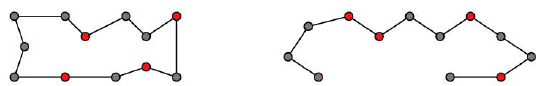
\includegraphics[width=\textwidth]{./img/4.png}

        \textcolor{blue}{\textbf{Megj:}} Az ábrán látható Petersen-gráfnak (sok más mellett) két érdekes tulajdonsága van. 

            \begin{enumerate}
                \item Teljesíti a fenti szükséges feltételt. 
                    \begin{enumerate}
                        \item Tegyük fel, hogy külső körből $k_1$, a belsőből $k_2$ csúcsot hagytunk el. Ha $k_1 = 0$ vagy $k_2 = 0$, akkor a gráf összefüggő marad. Különben a kölső kör legfeljebb $k_1$, a belső pedig legfeljebb $k_2$ részre esik szét, vagyis összesen legfeljebb $k_1 + k_2$ komponens létezik. \\ 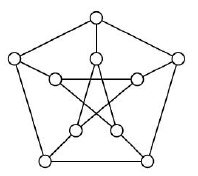
\includegraphics[width=0.2\textwidth]{./img/5.png}
                    \end{enumerate}
                \item Nincs Hamilton-köre.
                    \begin{enumerate}
                        \setcounter{enumi}{1}
                        \item Ha lenne Hamilton-köre, akkor a Hamilton-kör éleit felváltva pirosra és zöldre tudnánk színezni. Ha a körön kívüli élek sárgák, akkor a 3-regularitás miatt minden csúcsból pontosan egy piros, sárga ill. zöld él indulna. Ha megpróbáljuk az éleket így kiszínezni, kiderül, hogy nem lehet. \\ 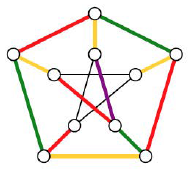
\includegraphics[width=0.2\textwidth]{./img/6.png}
                    \end{enumerate}
            \end{enumerate}
        
        A továbbiakban elégséges feltételeket fogunk látni Hamilton-kör létezésére. Ezek segítségével (szerencsés esetben) gyorsan és kétséget kizáróan tudjuk bizonyítani, hogy egy adott gráfnak van Hamilton-köre. Az elégséges feltétel vizsgálata azonban nem alkalmas arra, hogy egy gráf a Hamilton-körének hiányát igazoljuk.

        \textcolor{blue}{\textbf{Def:}} Legyen $G$ $n$-csúcsú, egyszerű gráf.

        Az $u,v \in V(G)$ csúcspár \textcolor{red}{gazdag}, ha $d(u) + d(v) \geq n$. A $G$ gráfra teljesül a \textcolor{red}{Dirac-feltétel}, ha $d(v) \geq \frac{n}{2} \forall v \in V(G)$-re. $G$-re igaz az \textcolor{red}{Ore-feltétel}, ha $G$ bármely két nem szomszédos csúcsa gazdag párt alkot.

        \textcolor{orange}{\textbf{Dirac tétele:}} $G$re igaz a Dirac-feltétel $\Rightarrow$ $G$-nek van H-köre.

        \textcolor{orange}{\textbf{Ore tétele:}} $G$-re igaz az Ore-feltétel $\Rightarrow$ $G$-nek van H-köre.

        \textcolor{blue}{\textbf{Megj:}} A Dirac-feltétel erősebb (többet kíván), mint az Ore. Ezért az Ore-tétel erősebb, mint a Dirac: gyengébb feltételből igazolja ugyanazt. Ezért az Ore-tétel bizonyítása a Dirac-tételt is igazolja.

        \item \textbf{A Chvátal-lezárt} 

        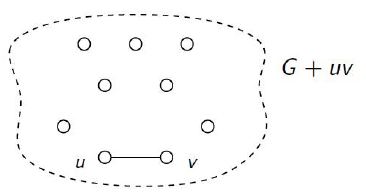
\includegraphics[width=0.2\textwidth]{./img/7.png}

        \textcolor{orange}{\textbf{Hízlalási lemma:}} Tegyük fel, hogy $G$ egyszerű gráf, és $(u,v)$ gazdag pár. ($G$-nek van Hamilton-köre) $\Longleftrightarrow$ ($G + uv$-nek van Hamiliton köre).

        \textcolor{blue}{\textbf{Megj:}} A hízlalási lemma jelentőségge az, hogy segít eldönteni azt, hogy van-e $G$-ben Hamilton-kör. Azt mondja ki ugyanis, hogy a gazdag párok közé $G$-be "ingyen" behúzhatunk éleket, u.i. ez nem változtat azon a tényen, hogy van vagy nincs Hamilton-kör a vizsgált gráfban. Megtehetjük tehát, hogy a lemma segítségével addig húzunk be éleket a gráfba, amíg lehet. Ha az így adódó $\overline{G}$ Chvátal-lezártban találunk Hamilton-kört, akkor $G$-nek is bizonyosan van Hamiliton-köre. Ha pedig $\overline{G}$ nem tartalmaz Hamilton-kört, akkor persze $G$-nek nincs Hamilton-köre.

        \textcolor{green}{\textbf{Biz:}} $\Rightarrow$: Láttuk. \checkmark $\Leftarrow$: Legyen $C$ a $G + uv$ Hamilton-köre. Ha $uv \notin C$, akkor $C$ a $G$-nek is Hamilton-köre, kész vagyunk. Ha viszont $uv \in C$, akkor $C-uv$ a $G$ egy Hamilton-útja. Legyen ez a Hamilton-út $u = v_1, v_2, \dots, v_n = v$. Legyen $A:=N(v) = \{v_i:vv_i \in E(G)\}$ a $v$ szomszédainak halmaza, és legyen $B: = \{v_{i-1} : uv_i \in E(G)\}$ az $u$ szomszédait a Hamilton-úton megelőző csúcsok halmaza.

        Világos, hogy $v \notin A$ és $v \notin B$, így $|A \cup B| \leq n-1$. Mivel $(u,v)$ gazdag pár, ezért $|A|+|B| = d(u)+d(v) \geq n$. Ezek szerint $A \cap V \neq \emptyset$, legyen pl. $v_i \in A \cap B$. Ekkor $v_1, v_2, \dots, v_i, v_n, v_{n-1}, \dots, v_{i+1}, v_1$ a $G$ egy Hamilton-köre. 

        \textcolor{orange}{\textbf{Ore tétele:}} Ha $G$ bármely két nemszomszédos csúcsa gazdag párt alkot, akkor $G$-nek van Hamilton-köre.

        \textcolor{green}{\textbf{Biz:}} A hízlalási lemma alapján $G$ bármely két nemszomszédos csúcsát "ingyen" összeköthetjük. Így $G$ Chátal-lezártja a $\overline{G} = K_n$ teljes gráf. Mivel $K_n$-nek van H-köre, ezért $G$-nek is van. 

        \textcolor{orange}{\textbf{Dirac-tétele:}} Ha $\delta(G) \geq \frac{|V(G)|}{2}$, akkor $G$-nek van Hamilton-köre.

        \textcolor{green}{\textbf{Biz:}} $G$ bármely két csúcsa gazdag párt alkot, ezért $G$-re teljesül az Ore-feltétel. Az Ore-tétel miatt $G$-nek van Hamilton-köre. 

    \end{itemize}

\end{document}